\documentclass[twocolumn]{article}

% if you need to pass options to natbib, use, e.g.:
%     \PassOptionsToPackage{numbers, compress}{natbib}
% before loading neurips_2020

% ready for submission
% \usepackage{neurips_2020}

% to compile a preprint version, e.g., for submission to arXiv, add add the
% [preprint] option:
%     \usepackage[preprint]{neurips_2020}

% to compile a camera-ready version, add the [final] option, e.g.:
%     \usepackage[final]{neurips_2020}

% to avoid loading the natbib package, add option nonatbib:
     \usepackage[final, nonatbib]{neurips_2020}
     \usepackage[ruled,vlined]{algorithm2e}

\usepackage[
backend=biber,
style=numeric,
sorting=none
]{biblatex}
\addbibresource{refs.bib}


\usepackage[utf8]{inputenc} % allow utf-8 input
\usepackage[T1]{fontenc}    % use 8-bit T1 fonts
\usepackage{hyperref}       % hyperlinks
\usepackage{url}            % simple URL typesetting
\usepackage{booktabs}       % professional-quality tables
\usepackage{amsfonts}       % blackboard math symbols
\usepackage{nicefrac}       % compact symbols for 1/2, etc.
\usepackage{microtype}      % microtypography
\usepackage[dvipsnames]{xcolor}
\usepackage{graphicx}
\usepackage{amsmath}
\usepackage{mathtools}
\usepackage{lipsum}
\usepackage{wrapfig}
\usepackage{xcolor}
\usepackage{subcaption}
\usepackage{multirow}
\usepackage{float}
\usepackage{stfloats}
\usepackage{amsthm}
\DeclareMathOperator*{\argmax}{arg\,max}
\DeclareMathOperator*{\argmin}{arg\,min}

\title{Road Segmentation Report}
%\title{Natural Language Retrieval For Language Grounding in Reinforcement Learning}
%\title{Peruse The Loathsome Enchidirion}
%\title{Know Where To Look}
% The \author macro works with any number of authors. There are two commands
% used to separate the names and addresses of multiple authors: \And and \AND.
%
% Using \And between authors leaves it to LaTeX to determine where to break the
% lines. Using \AND forces a line break at that point. So, if LaTeX puts 3 of 4
% authors names on the first line, and the last on the second line, try using
% \AND instead of \And before the third author name.

\author{
  Shabnam Ghasemirad\\
  \texttt{sghasemirad} \\
  % Affiliation \\
  % Address \\
  % \texttt{email} \\
   \And
  Harish Rajagopal \\
  \texttt{hrajagopal} \\
  % Affiliation \\
  % Address \\
  % \texttt{email} \\
   \And
  Ali Gorji \\
  \texttt{agorji} \\
  % Affiliation \\
  % Address \\
  % \texttt{email} \\
   \And
  Johannes Dollinger \\
  \texttt{jdollinger} \\
  % Affiliation \\
  % Address \\
  % \texttt{email} \\
}
\begin{document}

\twocolumn[\maketitle]

\section{Introduction} \label{intro}
The saying goes: "All roads lead to Rome." Were that the case, then the task of road segmentation would be pretty easy. But alas, it is not. Road segmentation concerns itself with automatically detecting roads and non-roads in bird's-eye view images, thus falling into the field of semantic segmentation in computer vision. Exemplary applications are the automatic generation of maps for navigation systems, which otherwise would have to be annotated by hand.

Previous models~\cite{bastani2018roadtracer, mattyus2017deeproadmapper, kaiser2017learning} are both very data-hungry and biased for straight road segments. The dataset in this work consists of 100 training images of $400 \times 400$ pixels and 96 test images with $608 \times 608$ pixels. This dataset is relatively small and also very noisy. To tackle the noise issue, we manually cleaned the data.

Our approach to the task combines a U-Net~\cite{unet} with Contrastive Learning~\cite{chopra2005learning} and a sequence of data augmentations~\cite{lecun1998gradient}.
In the post-processing step, we then apply Graph Cut ~\cite{graphcut} and a novel algorithm called Simple Physarum Polycephalum (Section~\ref{novelties:spp})\footnote{A documented implementation can be found on: \href{https://github.com/rharish101/CIL-Project}{https://github.com/rharish101/CIL-Project}}.
Section~\ref{novelties:scrapped} discusses multiple novelties that we attempted but decided to scrap due to no significant improvements over the baseline.

\section{Baseline}\label{section:baselines}
UNET baseline.
Also mention of GAN

\section{Novelties}\label{section:novelties}
One of the main observations in our baselines predictions was the patchy nature of classifications, as it did not produce coherent streets in most cases. When looking directly at the output probabilities, it was similar to a grey-scale image of the input. Thus the model was only focusing on texture instead of shape. Out novelties tried to remedy this by including inductive biases about shape in out classification.

\subsection{Deformations}

\subsection{Contrastive Learning in Bottleneck}

\subsection{UNET bottleneck}
In the U-Net architecture, the downsampling at each depth is done using max-pooling.
However, if the image size is too large, the layers might miss the global information at the lowest depth.
Hence, we experiment by using global average pooling at the lowest depth.
This enforces a bottleneck that captures a single scalar for the entire image in each channel.
This is done to capture global information from the entire image irrespective of the image size.


\subsection{Scrapped Novelties}
    This section gives an overview of the novelties that were tried, but didn't improve the model.

    Learned Ensemblers, Slime, Soft dice loss, GNN, CRF, Graph cuts. Soft dice loss (or maybe mention that in baseline)

    \subsubsection{GAN}
    The outputs of the baseline model are often not as smooth and continuous as the ground truth.
Thus, we use a GAN~\cite{gan} as a ``learned'' loss to enforce smoothness on a pixel-level.

Our baseline model is treated as the generator.
We add a patch discriminator~\cite{pix2pix} that has the same architecture as the left half of the baseline model.
We don't use a regular discriminator, since we want the discriminator to attend to the high-frequency output textures, which are better captured by image patches.
The outputs of the layer at the lowest depth gives us the discriminator's predictions per patch (here each patch is of size $32 \times 32$).
A global average pooling layer then converts all of the predictions into a single prediction for the image.

We use the Wasserstein~\cite{wgan} loss to train the network.
Additionally, we add spectral normalization~\cite{spectral-norm} to the weights of the discriminator to enforce the Lipschitz continuity constraint for the Wasserstein loss.

We observed that the improvements with the GAN are not substantial enough.
Further, it also increases the computation time.
Hence, we do not use this novelty in our final model.



\section{Experiments}\label{section:experiments}
We ran all the experiments using Adam optimizer with the learning rate of $10^{-4}$ and the weight decay of $5*10^{-6}$. We used Binary Cross Entropy as our primary loss function, summed up with the Contrastive Shape loss in the Contrastive Learning experiments.  We did all the preliminary experiments using 80 percent of the data to train for $3'000$ epochs and the rest for validation. In the final run, however, we used all the labeled data and trained the model for [?] epochs. All the random seeds are set to a fixed number to ensure the reproducibility of the results.

\section{Results}\label{section:results}
\begin{figure*}[b]
    \centering
    \begin{subfigure}{.5\textwidth}
        \centering
        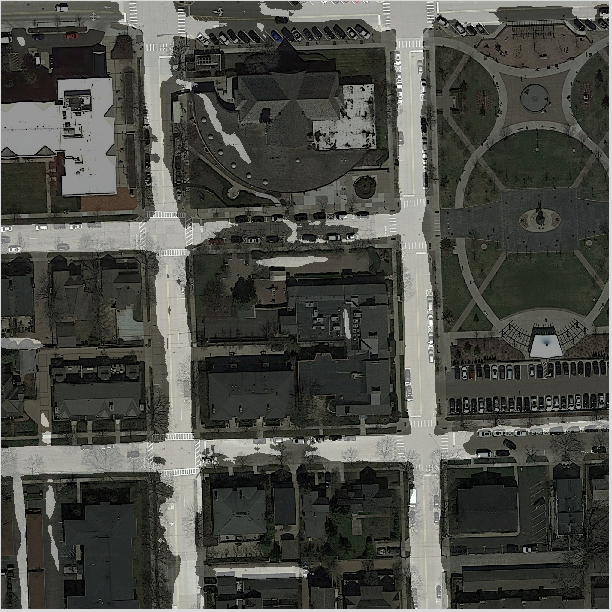
\includegraphics[width=.65\linewidth]{images/baseline_test_136.png}
        \caption{Baseline}%
        \label{fig:res_before}
    \end{subfigure}%
    \begin{subfigure}{.5\textwidth}
        \centering
        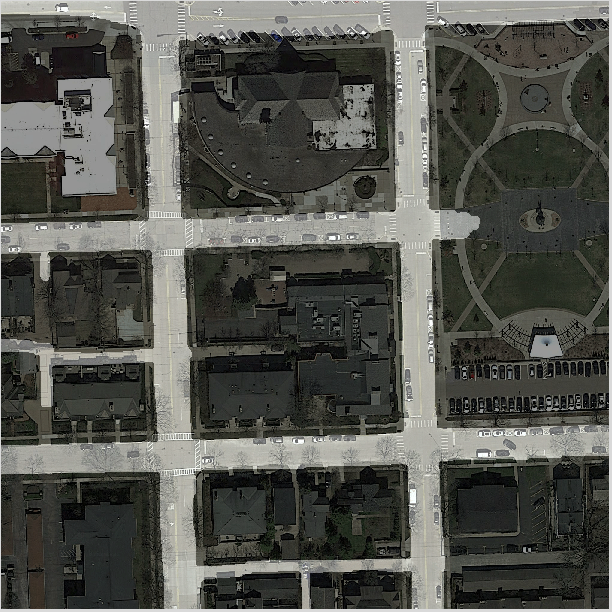
\includegraphics[width=.65\linewidth]{images/final_test_136.png}
        \caption{Final}%
        \label{fig:res_after}
    \end{subfigure}
    \caption{%
        Comparison of the baseline model with our final one.
        The output is binarized and overlaid on top of the input.
    }
\end{figure*}

Table \ref{results:metrics} highlights the results using the different novelties. The rows are arranged in the order of application --- we start with the baseline, and then apply our augmentations, contrastive learning, and so on.
Note that the test accuracy is calculated from the public Kaggle leaderboard, which uses the downsampled outputs.

\begin{table}[ht]
    \centering
    \caption{
        Comparison of results of all novelties.
        Each novelty is applied with all previous novelties.
    }%
    \label{results:metrics}
    \begin{tabular}{l r r r} 
        \toprule
        Method & Train Acc & Val Acc & Test Acc \\
        \midrule
        Baseline & 0.99132 & 0.96531 & 0.89714 \\ 
        + Aug & 0.97889 & 0.96470 & 0.91352 \\
        + CL & 0.97806 & 0.96230 & 0.91638 \\
        + Cleaned data & 0.97932 & 0.96394 & 0.92022 \\
        + Graph Cut & 0.97923 & 0.96327 & 0.91832 \\
        + SPP & 0.97936 & 0.96388 & \textbf{0.92144} \\
        \bottomrule
    \end{tabular}
\end{table}

Applying Graph Cut directly reduces the test accuracy, and decreases final accuracy as opposed to only applying SPP.
Still, we decide to submit this version, since the difference is minimal and the outputs show more sensible street classifications.
It is important to note, that these two post-processing algorithms are training data agnostic, and therefore they do not improve that metric.

Figure~\ref{fig:res_before} displays a sample output from the baseline model.
The corresponding image by our final model is shown in Figure~\ref{fig:res_after}.
It is visible how much our novelties improve over the baseline model, especially in the connectivity of streets.

\section{Conclusion}\label{section:conclusion}
Our solution includes different novelties at all steps of the machine learning pipeline.
First, the data is cleaned, then we apply a fine-tuned set of augmentations.
The training of our baseline is enriched with contrastive learning, and the outputs go through a post-processing pipeline consisting of Graph Cuts and SPP.

Two of our main novelties are SPP and contrastive learning for shape bias.
SPP makes clever use of the inductive biases of the road segmentation task.
On the other hand, the contrastive learning approach for inducing shape bias is a general approach that can be applied to any CNN-based model to reduce texture bias.

Our approach highlights the strength of both neural and non-neural approaches.
An avenue for future improvements is more fluently linking the different steps into a jointly learned pipeline to enable signal propagation between the final output metrics and the parameters of our core CNN.
Another avenue is to investigate how the proposed novelties can be applied to tasks other than road segmentation.

\newpage

\small
\printbibliography{}

\appendix

\section{Architecture}\label{appendix:architecture}
At each U-Net depth, we use a block of two 2D convolution layers with residual connections between the inputs and the block outputs.
Each 2D convolution layer is preceded by dropout~\cite{dropout} and succeeded by batch normalization~\cite{batch-norm} followed by a leaky ReLU activation function.
If the number of channels changes, then the skip connection has a $1 \times 1$ 2D convolution layer to transform the channels in the inputs.
Otherwise, the skip connection is an identity function.

Initially, the three RGB channels are transformed into $c_1$ channels.
At every depth, the number of channels increases by a factor of 2, until it reaches a fixed upper cap ($c_\mathrm{max}$).%chktex 35

Refer to Table~\ref{tab:unet-hyper-params} for further architecture-specific hyper-parameters.

\begin{table}[h]
    \centering
    \caption{U-Net architecture hyper-parameters}%
    \label{tab:unet-hyper-params}
    \begin{tabular}{l r}
        \toprule
        Hyper-parameter & Value \\
        \midrule
        U-Net depth & 6 \\
        Dropout & 0.1 \\
        Initial channels ($c_1$) & 64 \\
        Maximum channels ($c_\mathrm{max}$) & 1024 \\%chktex 35
        2D convolution kernel size & $3 \times 3$ \\
        2D convolution padding & SAME \\
        Leaky ReLU slope & 0.2 \\
        Max pooling kernel size & $2 \times 2$ \\
        \bottomrule
    \end{tabular}
\end{table}

\section{Augmentations}\label{appendix:augmentations}
We use the Albumentations~\cite{albumentations} library for all of our augmentations.


% -------- Class ----------------
\subsection{Augmentations for U-Net inputs}\label{appendix:augmentations-class}
Vanilla U-Net \cite{unet} uses elastic deformations as well as random crops as the augmentation set.
Our final sequence of augmentations is listed in Table~\ref{tab:augmentations-class}.
Each individual augmentation in the sequence is applied with the probability of $0.5$.

\begin{table*}
\centering
    \caption{
        Augmentations are applied sequentially in the following order with a probability of 0.5.
    }\label{tab:augmentations-class}
    \begin{tabular}{c l l}
        \toprule
        Class & Augmentation & Hyper-parameters \\
        \midrule
        \multirow{4}{*}{Rotation and Crop} & Random crop & crop size $= 256 \times 256$ \\
        & Random $90^{\circ}$ rotation & \\
        & Horizontal flip & \\
        & Vertical flip & \\
        \midrule
        \multirow{6}{*}{Color transformation} & \multirow[t]{2}{*}{Random brightness and contrast} & brightness $\sim U[-0.2, 0.2]$ \\
        & & contrast limit $\sim U[-0.2, 0.2]$ \\
        & \multirow[t]{2}{*}{Color jitter} & brightness, contrast $= 0.2$\\
        &  & hue, saturation $= 0.2$\\
        & \multirow[t]{2}{*}{Gaussian blur} & kernel size $k \sim \mathcal{U}\{3, 7\}$\\
        &  & standard deviation $\sigma = 0.3*((k-1)*0.5 - 1) + 0.8$\\
        \midrule
        \multirow{7}{*}{Shape deformation$^*$} & \multirow[t]{3}{*}{Elastic deformation} & $\alpha=1$ \\
        & & $\sigma=50$ \\
        & & $\alpha_{affine} \sim U[-50,50]$ \\
        & \multirow[t]{2}{*}{Grid distortion} & number of steps $=3$\\
        & & distortion $\sim U[-0.3, 0.3]$  \\
        & \multirow[t]{2}{*}{Optical distortion} & shift limit $\sim U[-0.05, 0.05]$\\
        & & Distortion limit: $\sim U[-0.05, 0.05]$  \\
        \bottomrule
        \multicolumn{3}{l}{\small * One of the three deformation transformations is randomly picked each time.}
    \end{tabular}
\end{table*}

% -------- Shape ----------------
\subsection{Augmentations for Contrastive Learning}\label{appendix:augmentations-shape}

When interpreting images in the frequency domain, shapes are generally low frequency components, while textures are generally high frequency components.
Since we need augmentations that preserve shape but change the texture, they need to either reduce high frequency components or distort them (e.g., by adding noise).
These are listed in Table~\ref{tab:augmentations-shape}.

\begin{table*}
    \caption{%
        Augmentations for contrastive learning.
        Each augmentation is applied in the following order with a probability of 0.5.
        The input image is assumed to be in $[0, 255]$.
    }\label{tab:augmentations-shape}
    \begin{tabular}{l l}
        \toprule
        Augmentation & Hyper-parameters \\
        \midrule
        \multirow[t]{2}{*}{Gaussian blur} & kernel size $k \sim \mathcal{U}\{3, 7\}$ \\
        & standard deviation $\sigma = 0.3*((k-1)*0.5 - 1) + 0.8$ \\
        Nearest-neighbour downscaling + upscaling & scale $\sim U[0.5, 0.75]$ \\
        JPEG compression & quality $\sim U[20, 50]$ \\
        \multirow[t]{2}{*}{Gaussian noise} & mean = 0 \\
        & variance $\in (10, 50)$ \\
        \multirow[t]{2}{*}{ISO noise} (using Poisson noise) & hue change angle $\sim U[3.6, 18]$ degrees \\
        & intensity $\sim U[0.1, 0.5]$ \\
        \bottomrule
    \end{tabular}
\end{table*}

\section{Hyperparameters}\label{appendix:hyper-params}
All the hyperparameters that are used in experiments are listed in Table \ref{tab:hyperparameters}. 
We use the same set of hyperparameters for all experiments.

\begin{table}[H]
    \centering
    \caption{The list of hyperparameters used for experiments.}%
    \label{tab:hyperparameters}
    \begin{tabular}{l l}
        \toprule
        Hyper-parameter & Value \\
        \midrule
        Minimum learning rate & $5 \times 10^{-5}$ \\
        Maximum learning rate & $10^{-4}$ \\
        Weight decay & $10^{-5}$ \\
        Number of epochs & $8000$ \\
        Random seeds\textsuperscript{*} & $0$ \\
        Train batch size & $24$ \\
        Binarization threshold & $0.5$ \\ 
        Shape loss coefficient ($\alpha_{shape}$) & $10^{-2}$ \\
        Shape loss softmax temperature ($\tau$) & $1$ \\
        GrabCut probable foreground threshold\textsuperscript{$\star$} & 0.1255 \\
        SPP change threshold\textsuperscript{$\star$} ($\lambda$) & 0.1 \\
        \bottomrule
        \multicolumn{2}{l}{\small * Specific to our codebase.} \\
        \multicolumn{2}{l}{\small $\star$ Thresholds are on image intensity in $[0, 1]$.}
    \end{tabular}
\end{table}

\end{document}
